% Options for packages loaded elsewhere
\PassOptionsToPackage{unicode}{hyperref}
\PassOptionsToPackage{hyphens}{url}
%
\documentclass[
]{book}
\usepackage{lmodern}
\usepackage{amssymb,amsmath}
\usepackage{ifxetex,ifluatex}
\ifnum 0\ifxetex 1\fi\ifluatex 1\fi=0 % if pdftex
  \usepackage[T1]{fontenc}
  \usepackage[utf8]{inputenc}
  \usepackage{textcomp} % provide euro and other symbols
\else % if luatex or xetex
  \usepackage{unicode-math}
  \defaultfontfeatures{Scale=MatchLowercase}
  \defaultfontfeatures[\rmfamily]{Ligatures=TeX,Scale=1}
\fi
% Use upquote if available, for straight quotes in verbatim environments
\IfFileExists{upquote.sty}{\usepackage{upquote}}{}
\IfFileExists{microtype.sty}{% use microtype if available
  \usepackage[]{microtype}
  \UseMicrotypeSet[protrusion]{basicmath} % disable protrusion for tt fonts
}{}
\makeatletter
\@ifundefined{KOMAClassName}{% if non-KOMA class
  \IfFileExists{parskip.sty}{%
    \usepackage{parskip}
  }{% else
    \setlength{\parindent}{0pt}
    \setlength{\parskip}{6pt plus 2pt minus 1pt}}
}{% if KOMA class
  \KOMAoptions{parskip=half}}
\makeatother
\usepackage{xcolor}
\IfFileExists{xurl.sty}{\usepackage{xurl}}{} % add URL line breaks if available
\IfFileExists{bookmark.sty}{\usepackage{bookmark}}{\usepackage{hyperref}}
\hypersetup{
  pdftitle={Data Visualization with PowerBI},
  pdfauthor={Mohamed Kassem},
  hidelinks,
  pdfcreator={LaTeX via pandoc}}
\urlstyle{same} % disable monospaced font for URLs
\usepackage{color}
\usepackage{fancyvrb}
\newcommand{\VerbBar}{|}
\newcommand{\VERB}{\Verb[commandchars=\\\{\}]}
\DefineVerbatimEnvironment{Highlighting}{Verbatim}{commandchars=\\\{\}}
% Add ',fontsize=\small' for more characters per line
\usepackage{framed}
\definecolor{shadecolor}{RGB}{248,248,248}
\newenvironment{Shaded}{\begin{snugshade}}{\end{snugshade}}
\newcommand{\AlertTok}[1]{\textcolor[rgb]{0.94,0.16,0.16}{#1}}
\newcommand{\AnnotationTok}[1]{\textcolor[rgb]{0.56,0.35,0.01}{\textbf{\textit{#1}}}}
\newcommand{\AttributeTok}[1]{\textcolor[rgb]{0.77,0.63,0.00}{#1}}
\newcommand{\BaseNTok}[1]{\textcolor[rgb]{0.00,0.00,0.81}{#1}}
\newcommand{\BuiltInTok}[1]{#1}
\newcommand{\CharTok}[1]{\textcolor[rgb]{0.31,0.60,0.02}{#1}}
\newcommand{\CommentTok}[1]{\textcolor[rgb]{0.56,0.35,0.01}{\textit{#1}}}
\newcommand{\CommentVarTok}[1]{\textcolor[rgb]{0.56,0.35,0.01}{\textbf{\textit{#1}}}}
\newcommand{\ConstantTok}[1]{\textcolor[rgb]{0.00,0.00,0.00}{#1}}
\newcommand{\ControlFlowTok}[1]{\textcolor[rgb]{0.13,0.29,0.53}{\textbf{#1}}}
\newcommand{\DataTypeTok}[1]{\textcolor[rgb]{0.13,0.29,0.53}{#1}}
\newcommand{\DecValTok}[1]{\textcolor[rgb]{0.00,0.00,0.81}{#1}}
\newcommand{\DocumentationTok}[1]{\textcolor[rgb]{0.56,0.35,0.01}{\textbf{\textit{#1}}}}
\newcommand{\ErrorTok}[1]{\textcolor[rgb]{0.64,0.00,0.00}{\textbf{#1}}}
\newcommand{\ExtensionTok}[1]{#1}
\newcommand{\FloatTok}[1]{\textcolor[rgb]{0.00,0.00,0.81}{#1}}
\newcommand{\FunctionTok}[1]{\textcolor[rgb]{0.00,0.00,0.00}{#1}}
\newcommand{\ImportTok}[1]{#1}
\newcommand{\InformationTok}[1]{\textcolor[rgb]{0.56,0.35,0.01}{\textbf{\textit{#1}}}}
\newcommand{\KeywordTok}[1]{\textcolor[rgb]{0.13,0.29,0.53}{\textbf{#1}}}
\newcommand{\NormalTok}[1]{#1}
\newcommand{\OperatorTok}[1]{\textcolor[rgb]{0.81,0.36,0.00}{\textbf{#1}}}
\newcommand{\OtherTok}[1]{\textcolor[rgb]{0.56,0.35,0.01}{#1}}
\newcommand{\PreprocessorTok}[1]{\textcolor[rgb]{0.56,0.35,0.01}{\textit{#1}}}
\newcommand{\RegionMarkerTok}[1]{#1}
\newcommand{\SpecialCharTok}[1]{\textcolor[rgb]{0.00,0.00,0.00}{#1}}
\newcommand{\SpecialStringTok}[1]{\textcolor[rgb]{0.31,0.60,0.02}{#1}}
\newcommand{\StringTok}[1]{\textcolor[rgb]{0.31,0.60,0.02}{#1}}
\newcommand{\VariableTok}[1]{\textcolor[rgb]{0.00,0.00,0.00}{#1}}
\newcommand{\VerbatimStringTok}[1]{\textcolor[rgb]{0.31,0.60,0.02}{#1}}
\newcommand{\WarningTok}[1]{\textcolor[rgb]{0.56,0.35,0.01}{\textbf{\textit{#1}}}}
\usepackage{longtable,booktabs}
% Correct order of tables after \paragraph or \subparagraph
\usepackage{etoolbox}
\makeatletter
\patchcmd\longtable{\par}{\if@noskipsec\mbox{}\fi\par}{}{}
\makeatother
% Allow footnotes in longtable head/foot
\IfFileExists{footnotehyper.sty}{\usepackage{footnotehyper}}{\usepackage{footnote}}
\makesavenoteenv{longtable}
\usepackage{graphicx,grffile}
\makeatletter
\def\maxwidth{\ifdim\Gin@nat@width>\linewidth\linewidth\else\Gin@nat@width\fi}
\def\maxheight{\ifdim\Gin@nat@height>\textheight\textheight\else\Gin@nat@height\fi}
\makeatother
% Scale images if necessary, so that they will not overflow the page
% margins by default, and it is still possible to overwrite the defaults
% using explicit options in \includegraphics[width, height, ...]{}
\setkeys{Gin}{width=\maxwidth,height=\maxheight,keepaspectratio}
% Set default figure placement to htbp
\makeatletter
\def\fps@figure{htbp}
\makeatother
\setlength{\emergencystretch}{3em} % prevent overfull lines
\providecommand{\tightlist}{%
  \setlength{\itemsep}{0pt}\setlength{\parskip}{0pt}}
\setcounter{secnumdepth}{5}
\usepackage{booktabs}
\usepackage{amsthm}
\makeatletter
\def\thm@space@setup{%
  \thm@preskip=8pt plus 2pt minus 4pt
  \thm@postskip=\thm@preskip
}
\makeatother
\usepackage[]{natbib}
\bibliographystyle{apalike}

\title{Data Visualization with PowerBI}
\author{Mohamed Kassem}
\date{2021-04-27}

\begin{document}
\maketitle

{
\setcounter{tocdepth}{1}
\tableofcontents
}
\hypertarget{intorduction}{%
\chapter{Intorduction}\label{intorduction}}

This course is intended for educational purposes \& preparing Data analysts for Exam DA-100: Analyzing Data with Microsoft Power BI : \textbf{Creating reports}

\begin{itemize}
\item
  All the needed resources to follow along can be found here \url{https://github.com/Mkassem16/NycTaxiPBI}.
\item
  Creating basic PowerBI reports knowledge is prerequisite for this course.
\end{itemize}

\textbf{By the end of this course Data Analysts should be able to:}\\
+ Customize Report pages.\\
+ Decide for appropriate visualizations type.\\
+ To utilize PowerBI native visualizations.\\
+ Format and configure PowerBI native visuals.\\
+ Configure conditional formatting.\\
+ Import their own custom R or Python Visuals.\\
+ Utilize Slicers and Filters.\\
+ Adjust visuals for accessibility.\\
+ Configure automatic page refresh.\\
+ Create paginated reports.

\hypertarget{setting-and-objectives}{%
\chapter{Setting and Objectives}\label{setting-and-objectives}}

\hypertarget{setting}{%
\section{Setting}\label{setting}}

The New York City Taxi and Limousine Commission (TLC), created in 1971, is the agency responsible for licensing and regulating New York City's Medallion (Yellow) taxi cabs. Over 200,000 TLC licensees complete approximately 1,000,000 trips each day.

For the sake of educational purposes Data Analysts should think of an Imaginary situation where NYC TLC has asked them to prepare a PowerBI report for their c-suite executives and decision managers to better under stand their monthly operations in general and track their daily and monthly KPIs.

\hypertarget{objectives}{%
\section{Objectives}\label{objectives}}

\hypertarget{general}{%
\subsection{General}\label{general}}

\begin{itemize}
\tightlist
\item
  Creating an easy to read and understand descriptive dashboard.
\item
  Quick one look dynamic status updates.
\item
  Tracking daily and weekly KPIs.
\item
  Understanding revenue breakdown.
\end{itemize}

\hypertarget{requested}{%
\subsection{Requested}\label{requested}}

\begin{itemize}
\tightlist
\item
  Is there a specific day of week that NYC TLC should deploy more licensees?
\item
  Is there a specific time of day that NYC TLC should deploy more licensees?
\end{itemize}

\hypertarget{extra}{%
\subsection{Extra}\label{extra}}

\begin{itemize}
\tightlist
\item
  Mining for relations between trip duration, distance and fare.
\end{itemize}

\hypertarget{data}{%
\chapter{Data}\label{data}}

Data is publicly available at \url{https://www1.nyc.gov/site/tlc/about/tlc-trip-record-data.page}

Please Find Data catalog explaining columns and categories here: \url{https://github.com/Mkassem16/NycTaxiPBI/blob/main/data/data_dictionary_trip_records_yellow.pdf}

For the purpose of building a demonstration dashboard, I extracted a sample of 10,000 rows of 2020 data. This sample dataset is hosted publicly on Google Cloud storage and can be queried directly from PowerBi.
\url{https://storage.googleapis.com/powerbi_datacamp/nyc_taxi_db.csv}

\begin{Shaded}
\begin{Highlighting}[]
\KeywordTok{glimpse}\NormalTok{(df)}
\end{Highlighting}
\end{Shaded}

\begin{verbatim}
## Rows: 10,018
## Columns: 17
## $ vendor_id           <dbl> 1, 1, 2, 1, 2, 1, 4, 2, 1, 2, 1, 2, 2, 2, 2, 2,...
## $ pickup_datetime     <dttm> 2021-03-27 12:47:16, 2021-06-10 19:02:02, 2021...
## $ dropoff_datetime    <dttm> 2021-03-27 13:39:54, 2021-06-10 19:31:53, 2021...
## $ passenger_count     <dbl> 1, 1, 1, 1, 2, 1, 1, 1, 1, 1, 1, 1, 1, 2, 1, 2,...
## $ trip_distance       <dbl> 2.70, 15.10, 7.92, 6.50, 6.44, 10.00, 7.24, 36....
## $ rate_code           <dbl> 1, 1, 1, 1, 1, 1, 1, 5, 1, 1, 1, 1, 1, 1, 1, 1,...
## $ store_and_fwd_flag  <chr> "N", "N", "N", "N", "N", "N", "N", "N", "N", "N...
## $ payment_type        <dbl> 1, 1, 1, 1, 1, 1, 1, 1, 1, 1, 1, 1, 1, 1, 1, 1,...
## $ fare_amount         <dbl> 29.0, 42.0, 26.0, 22.5, 24.5, 29.0, 22.0, 83.5,...
## $ extra               <dbl> 0.0, 0.0, 0.5, 0.5, 0.5, 0.5, 0.5, 0.0, 0.0, 0....
## $ mta_tax             <dbl> 0.5, 0.5, 0.5, 0.5, 0.5, 0.5, 0.5, 0.0, 0.5, 0....
## $ tip_amount          <dbl> 5.95, 12.10, 5.46, 4.75, 3.87, 6.05, 4.66, 21.5...
## $ tolls_amount        <dbl> 0.00, 5.76, 0.00, 0.00, 0.00, 0.00, 0.00, 23.76...
## $ imp_surcharge       <dbl> 0.3, 0.3, 0.3, 0.3, 0.3, 0.3, 0.3, 0.3, 0.3, 0....
## $ total_amount        <dbl> 35.75, 60.66, 32.76, 28.55, 29.67, 36.35, 27.96...
## $ pickup_location_id  <dbl> 68, 138, 261, 262, 261, 100, 7, 132, 264, 170, ...
## $ dropoff_location_id <dbl> 162, 88, 41, 231, 162, 127, 53, 265, 264, 236, ...
\end{verbatim}

\hypertarget{dataset}{%
\chapter{Dataset}\label{dataset}}

\emph{Dataset} in PowerBI vocabulary is: the set of queries that the user will perform in order to import all of his data tables and all the transformations that will take place before data can be ready for the model and visualization.

\textbf{We will perform 2 queries to create 2 data tables:}

\begin{itemize}
\tightlist
\item
  Table 1 (\textbf{nyc\_taxi\_21}) : will include NYC TLC data. \url{https://github.com/Mkassem16/NycTaxiPBI/blob/main/queries/nyc_taxi_21.pq}
\item
  Table 2 (\textbf{Calendar}) : Calendar table that will control the date dimension
  \url{https://github.com/Mkassem16/NycTaxiPBI/blob/main/queries/Calendar.pq}
\end{itemize}

\hypertarget{step-1}{%
\section{Step 1}\label{step-1}}

Getting data through Blank query
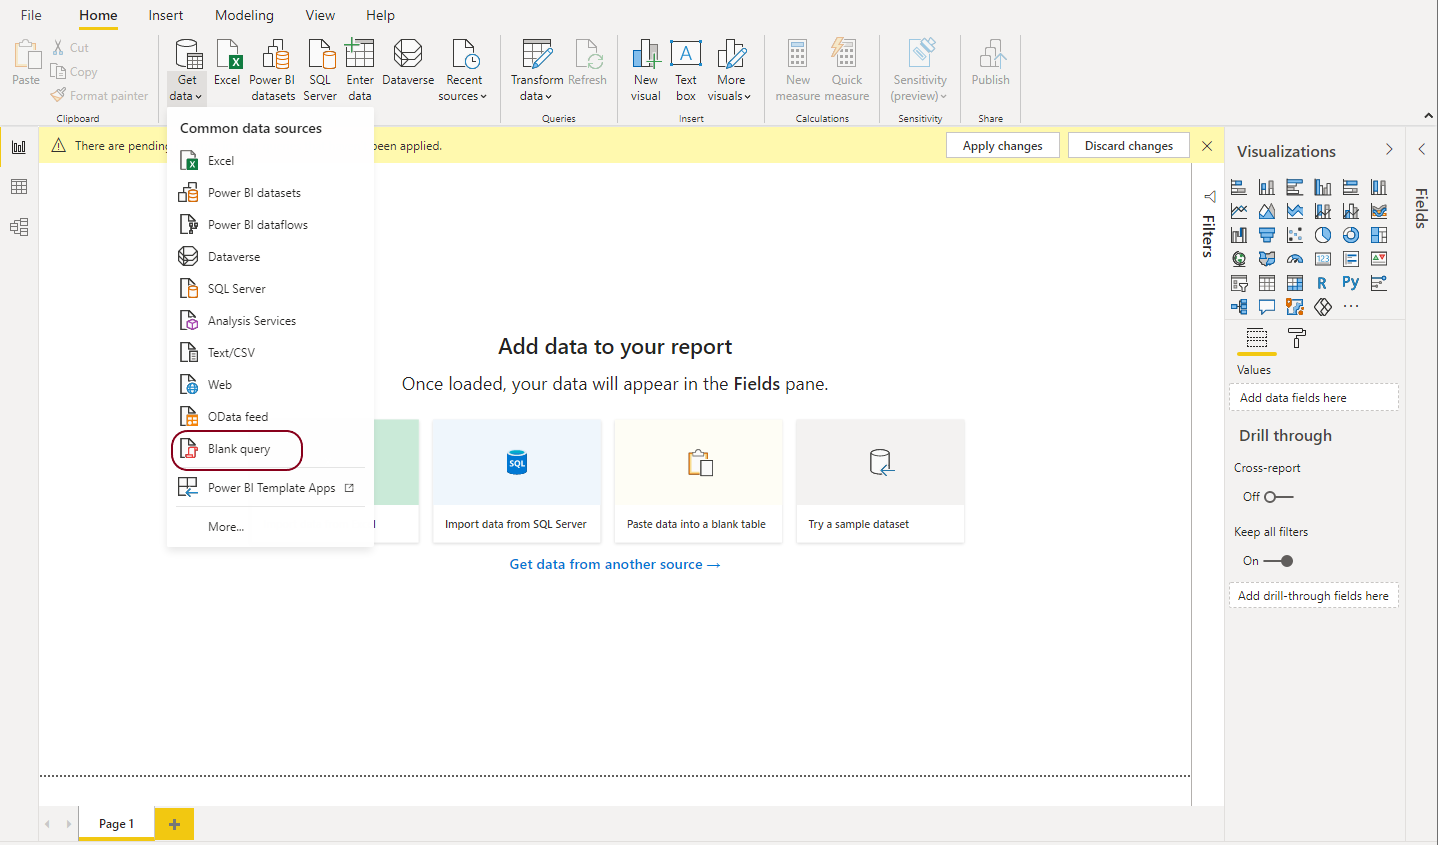
\includegraphics{assets/get_data.png}

\hypertarget{step-2}{%
\section{Step 2}\label{step-2}}

Choose Advanced editor
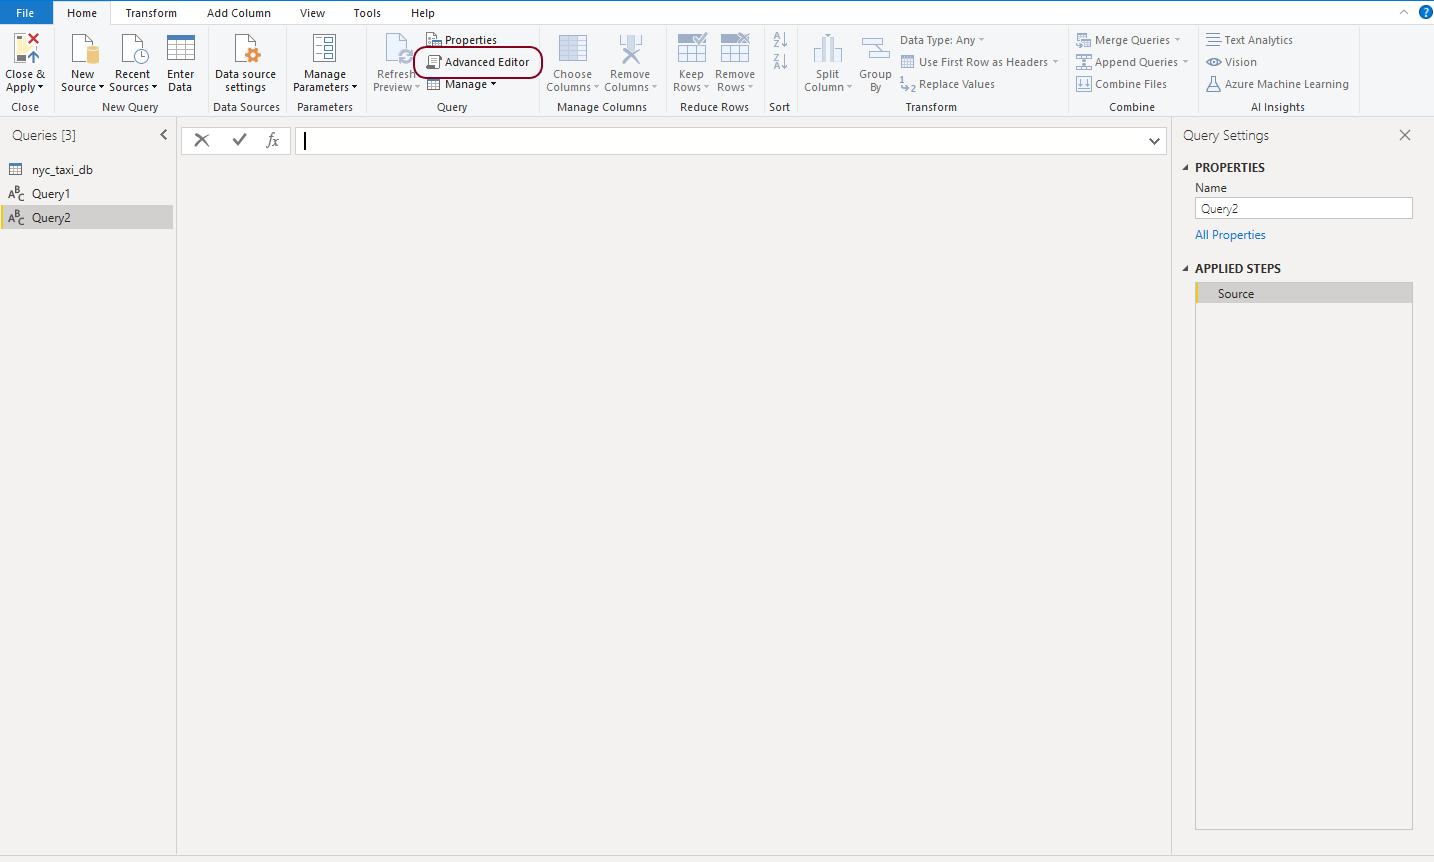
\includegraphics{assets/get_data2.png}

\hypertarget{step-3}{%
\section{Step 3}\label{step-3}}

Get the query of Table 1 from the provided link and paste it here instead of
what is already there
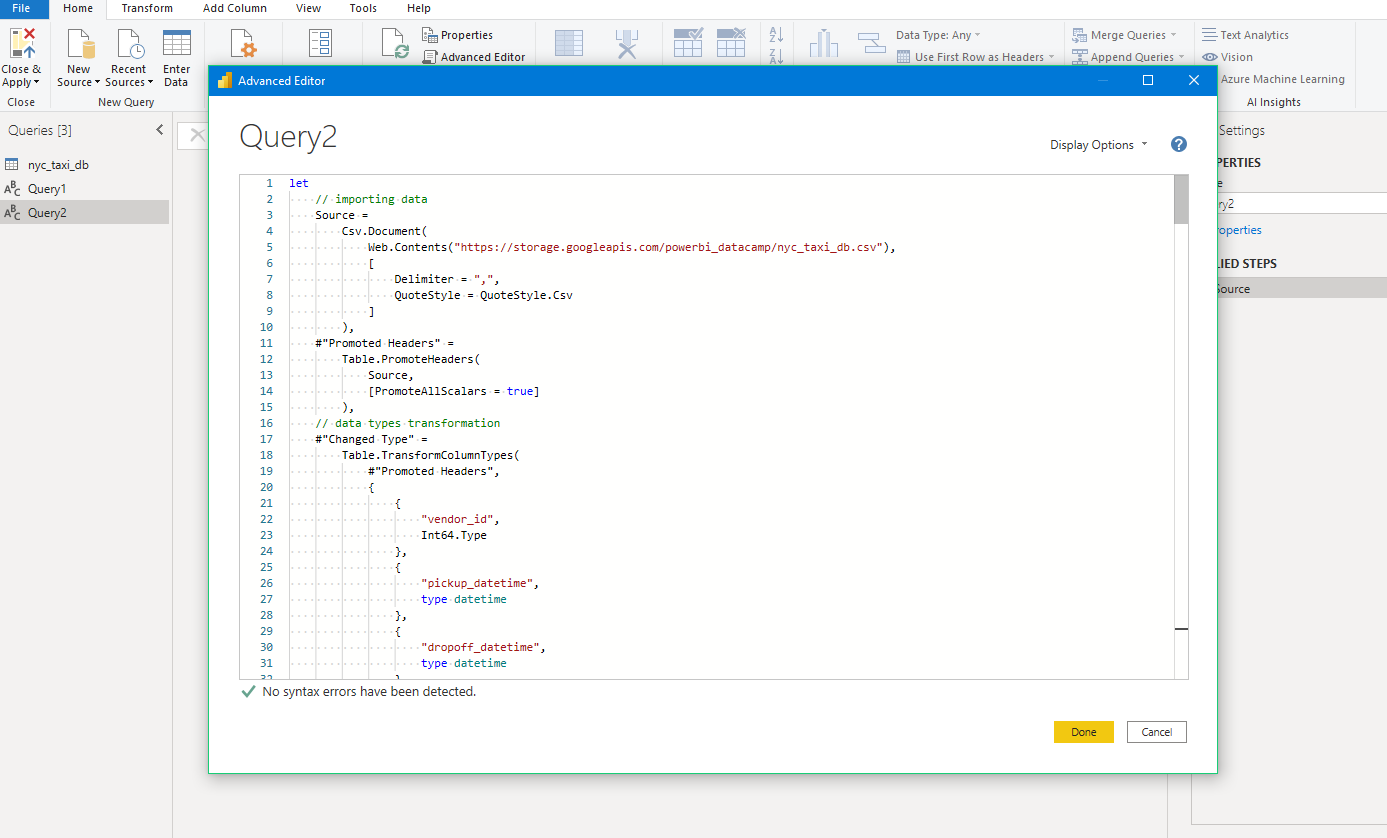
\includegraphics{assets/query_1.png}
\#\# Step 4

Make sure that query name is \textbf{nyc\_taxi\_21}
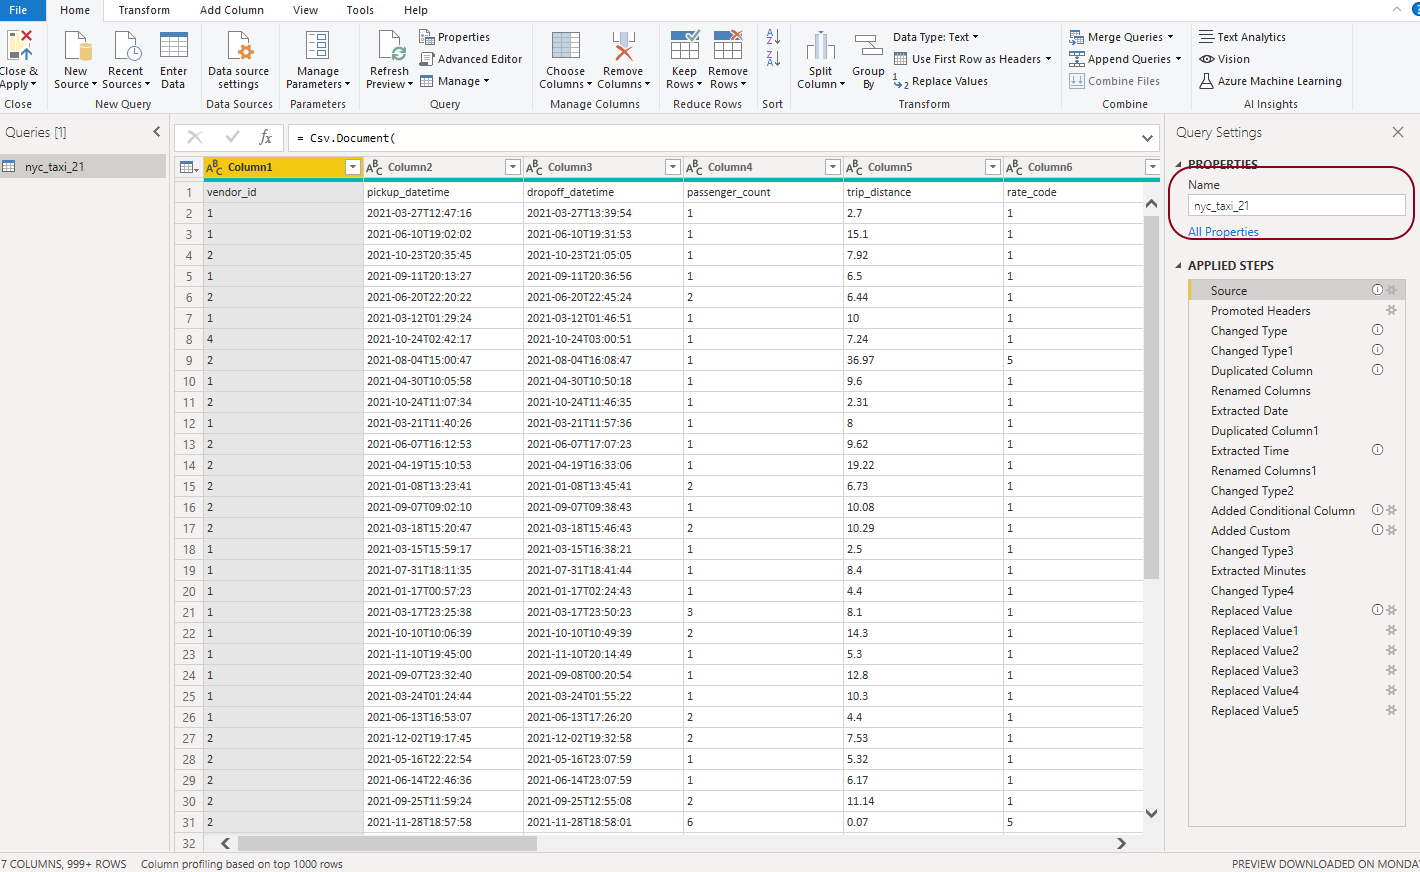
\includegraphics{assets/query_1b.png}

\hypertarget{step-5}{%
\section{Step 5}\label{step-5}}

Get the query of Table 2 from the provided link and paste it here instead of
what is already there
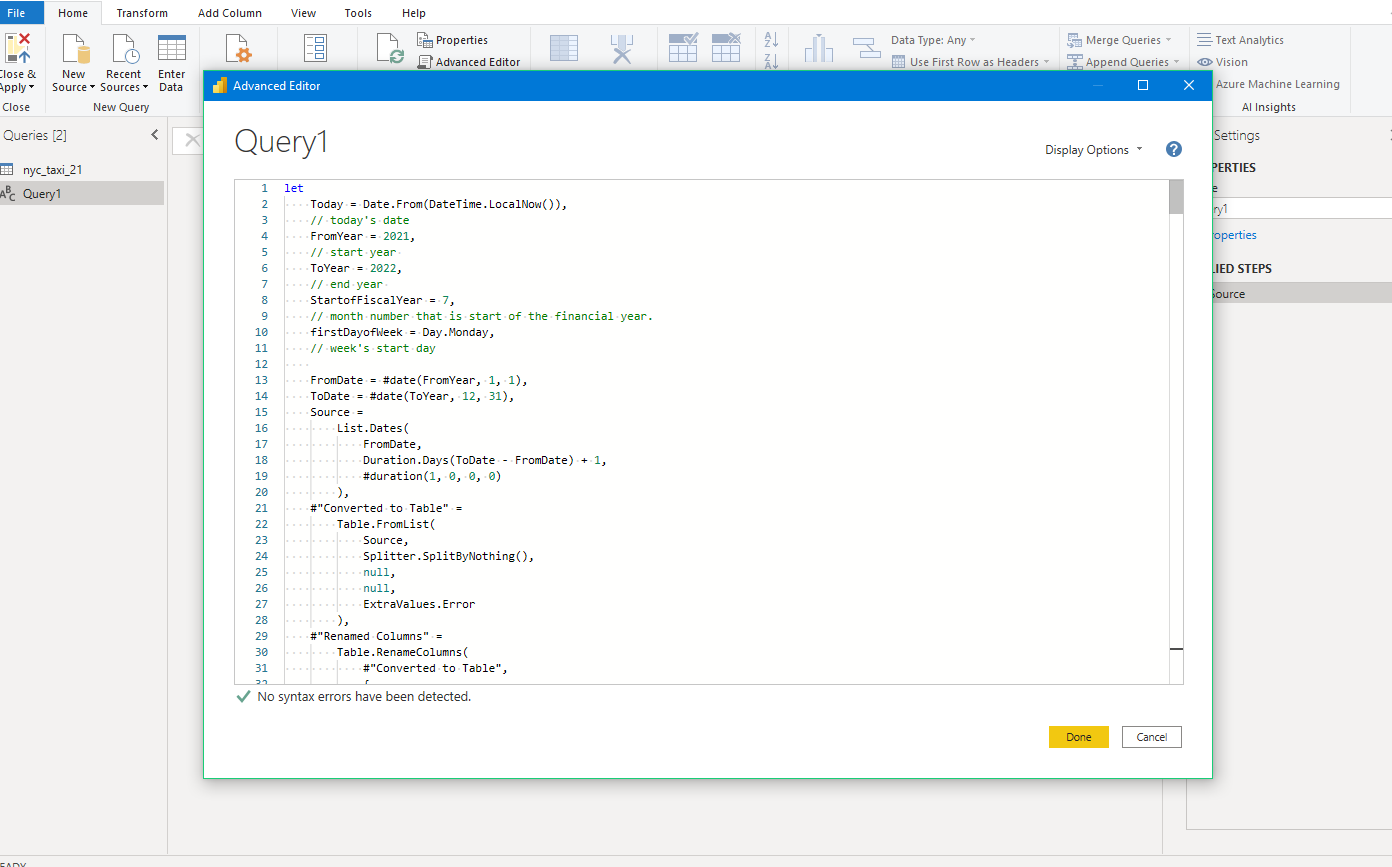
\includegraphics{assets/query_2.png}

\hypertarget{step-6}{%
\section{Step 6}\label{step-6}}

Make sure that query name is \textbf{Calendar}
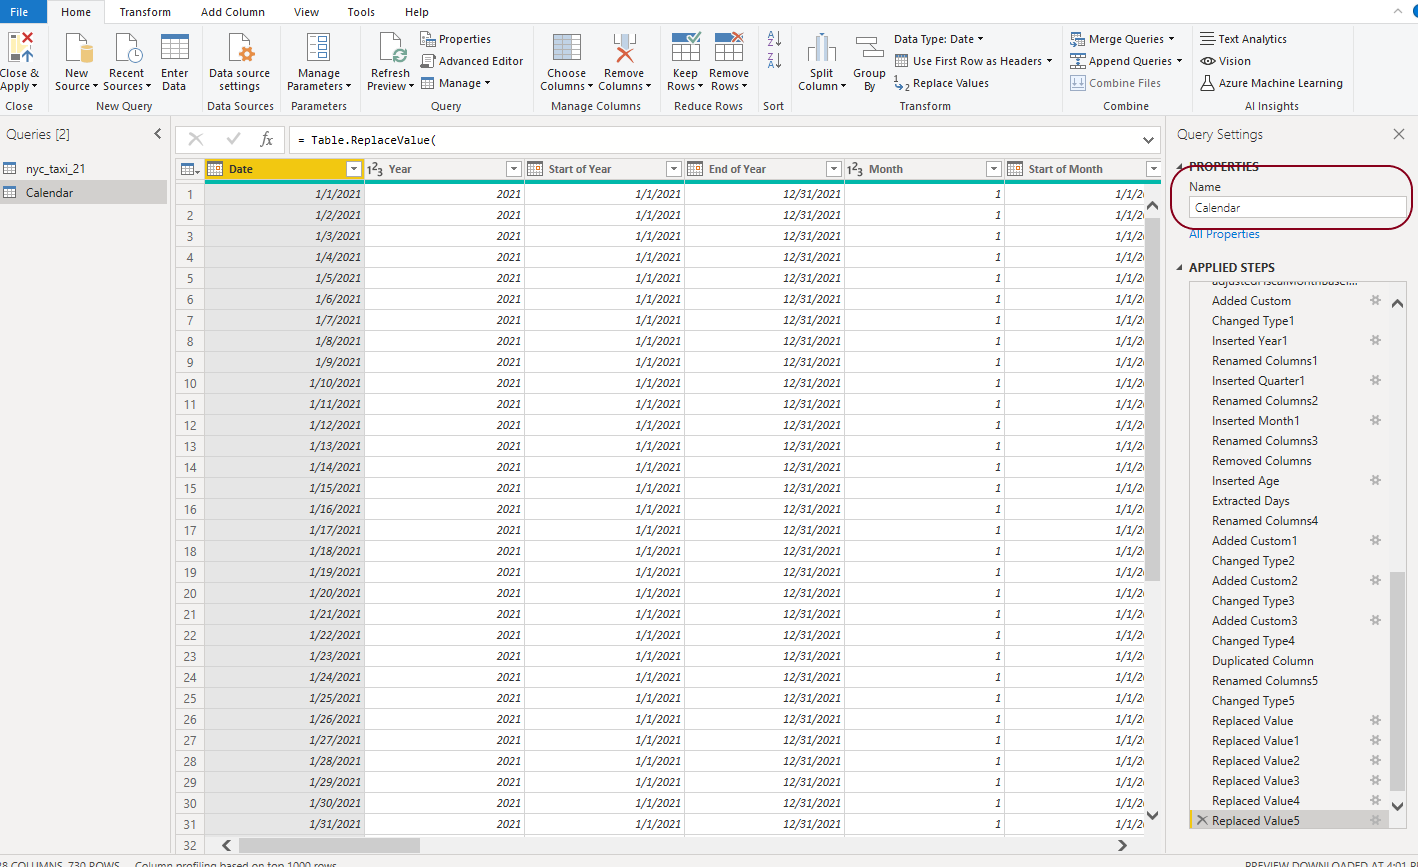
\includegraphics{assets/query_2b.png}

\hypertarget{step-7}{%
\section{Step 7}\label{step-7}}

Double check queries names as its important for Measures created through DAX,
Then click close \& apply
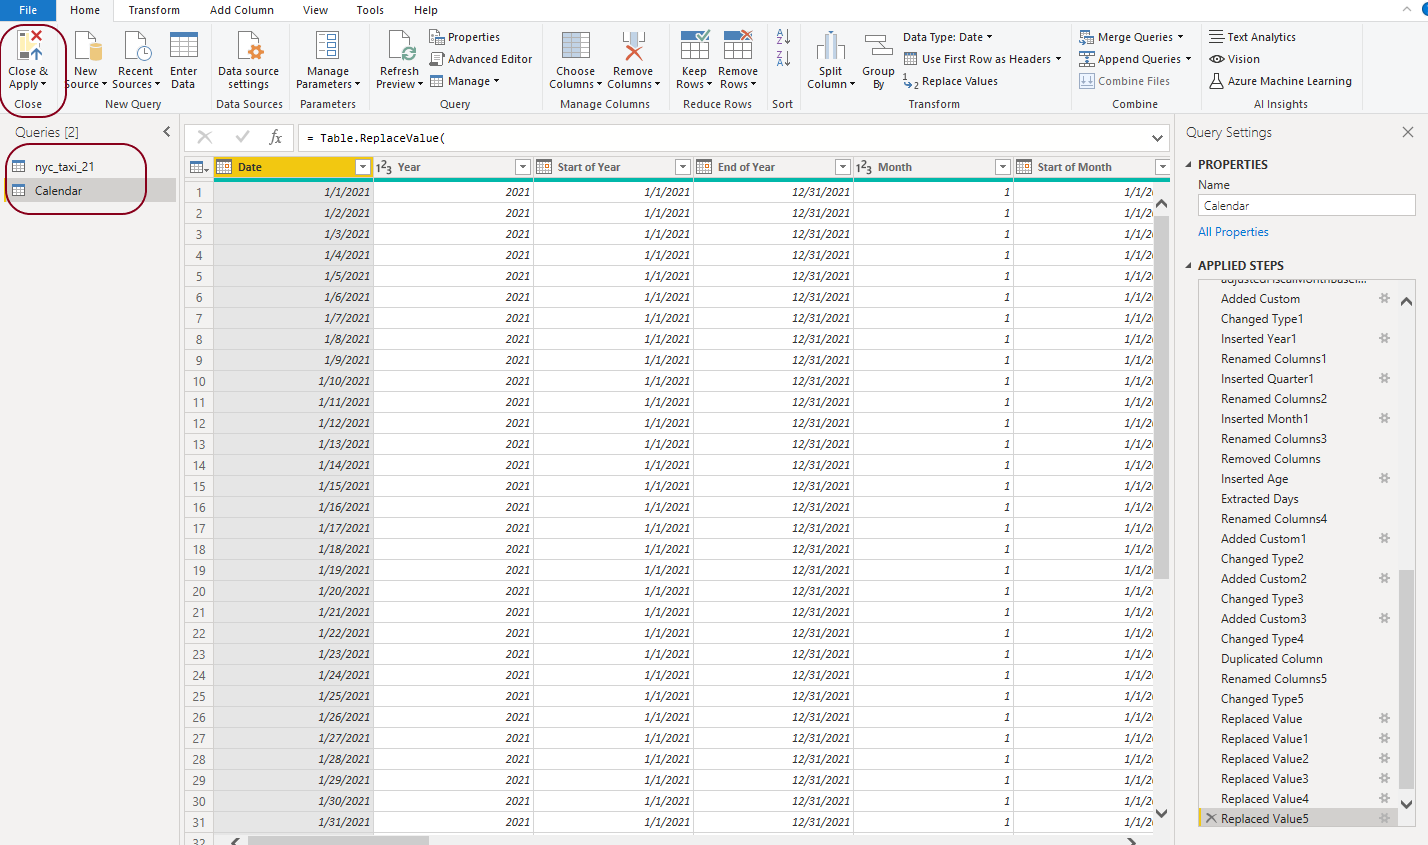
\includegraphics{assets/get_data3.png}

\hypertarget{datamodel}{%
\chapter{DataModel}\label{datamodel}}

\emph{Data Modeling} in PowerBI vocabulary is: the step of creating relations between tables before proceeding and building slicers and filters on our visuals we need to make sure that the relationships are with the right direction, cardinality and that they are active.

\textbf{We will create 1 relation between Calendar table and the data table}

\hypertarget{step-1-1}{%
\section{Step 1}\label{step-1-1}}

Navigate to data modeling view
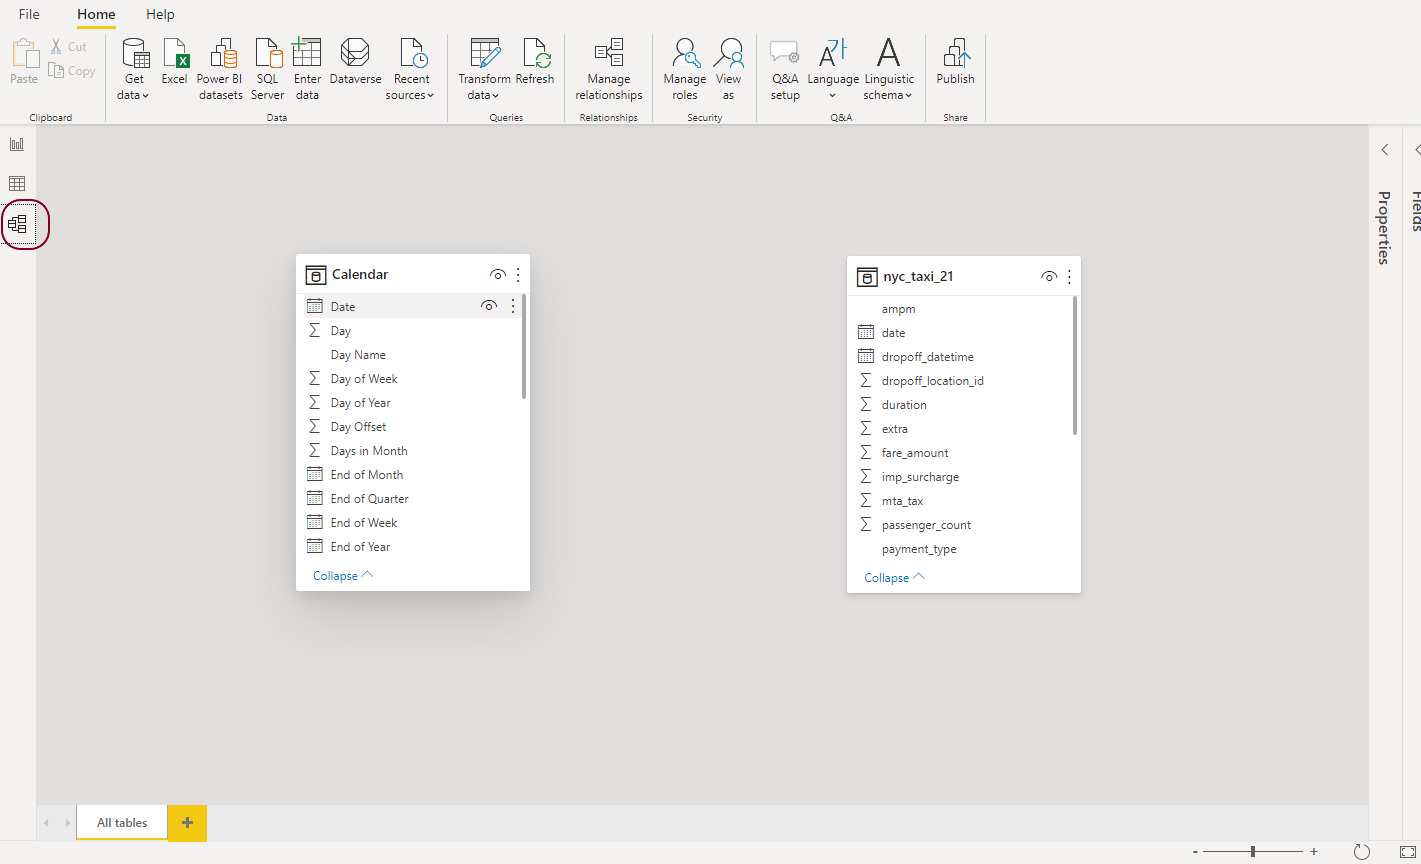
\includegraphics{assets/datamodel1.png}

\hypertarget{step-2-1}{%
\section{Step 2}\label{step-2-1}}

Click on manage relations
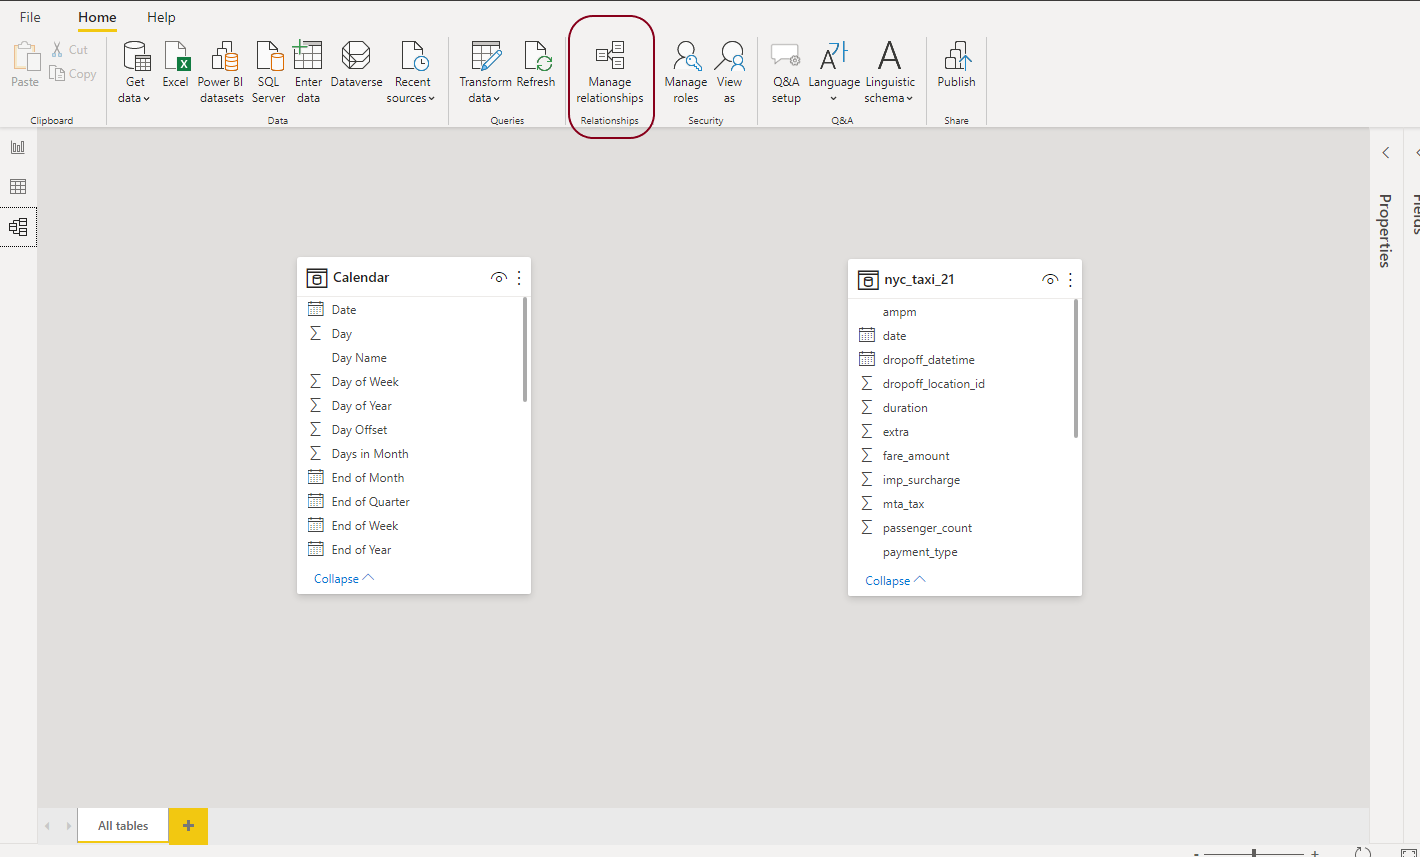
\includegraphics{assets/datamodel2.png}

\hypertarget{step-3-1}{%
\section{Step 3}\label{step-3-1}}

Create new relation and make sure of the following:

\begin{itemize}
\tightlist
\item
  Select the right tables\\
\item
  Select the right columns (by clicking on the column name in the display)\\
\item
  Select the right Cardinality (usually with Calendar tables its One to many)\\
\item
  Select the right direction (\textbf{Calendar} table to filter \textbf{nyc\_tax\_21} table)\\
  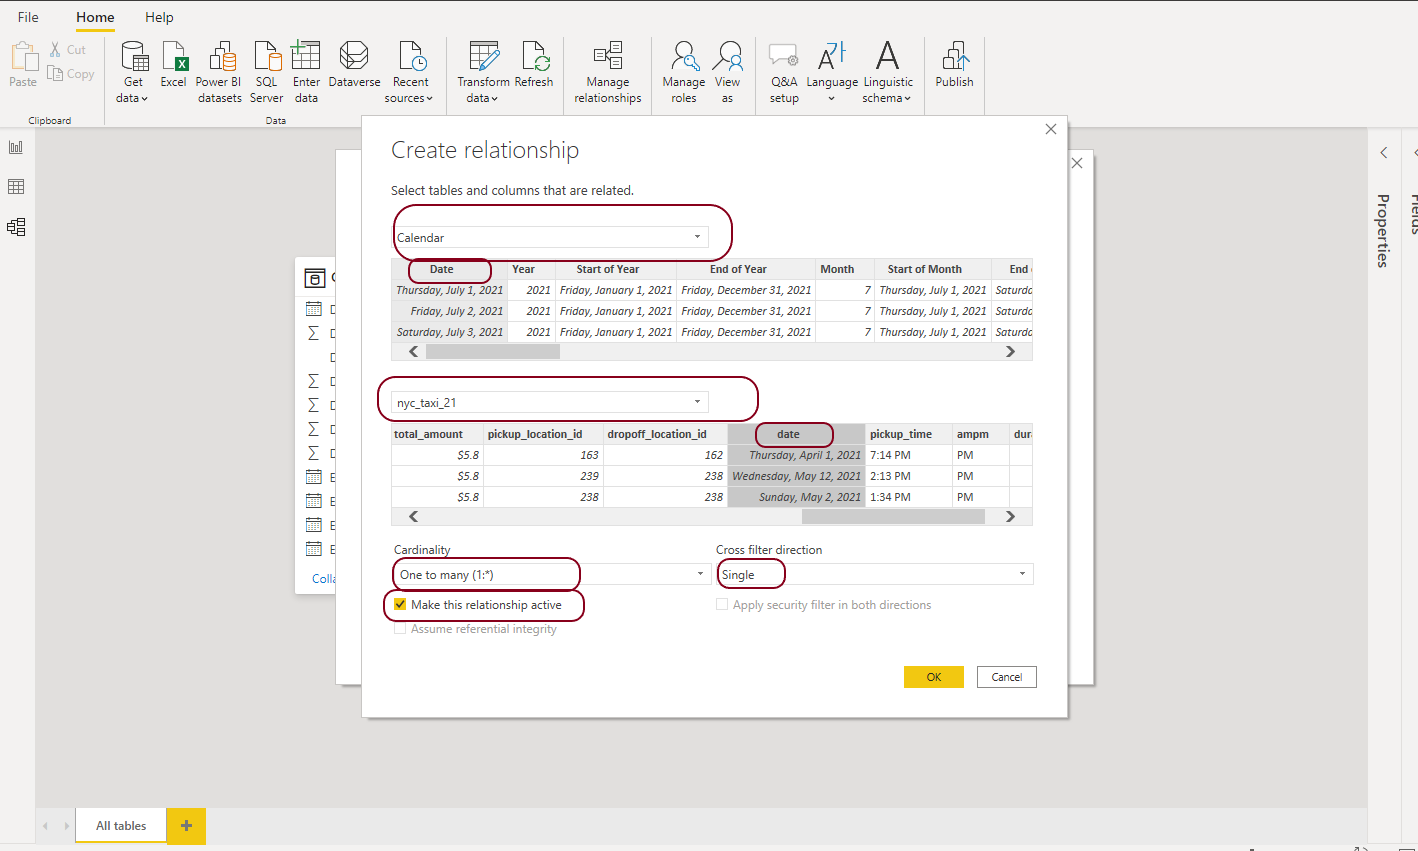
\includegraphics{assets/datamodel3.png}
\end{itemize}

\hypertarget{report-page}{%
\chapter{Report page}\label{report-page}}

We can start customizing report page by clicking on the format icon of the Visualization pane without choosing any visual.

\begin{figure}
\centering
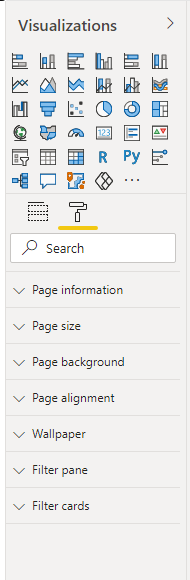
\includegraphics{assets/page_1.png}
\caption{format}
\end{figure}

\textbf{Options include:}

\hypertarget{information}{%
\section{information}\label{information}}

\hypertarget{size}{%
\section{Size}\label{size}}

\hypertarget{background}{%
\section{Background}\label{background}}

\hypertarget{alignment}{%
\section{Alignment}\label{alignment}}

\hypertarget{wallpaper}{%
\section{Wallpaper}\label{wallpaper}}

\hypertarget{visualization-types}{%
\chapter{Visualization types}\label{visualization-types}}

\hypertarget{comparison}{%
\section{Comparison}\label{comparison}}

\hypertarget{change-over-time}{%
\section{Change over time}\label{change-over-time}}

\hypertarget{ranking}{%
\section{Ranking}\label{ranking}}

\hypertarget{spatial}{%
\section{Spatial}\label{spatial}}

\hypertarget{part-to-whole}{%
\section{Part-to-whole}\label{part-to-whole}}

\hypertarget{distribution}{%
\section{Distribution}\label{distribution}}

\hypertarget{correlation}{%
\section{Correlation}\label{correlation}}

\hypertarget{single}{%
\section{Single}\label{single}}

\hypertarget{filter-slicer}{%
\section{Filter \& Slicer}\label{filter-slicer}}

\hypertarget{powerbi-native-visuals}{%
\chapter{PowerBI native visuals}\label{powerbi-native-visuals}}

\begin{figure}
\centering
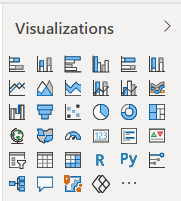
\includegraphics{assets/native1.png}
\caption{native}
\end{figure}

PowerBi offers a group of native visualizations that we will build most of the dashboard using them.

\hypertarget{comparison-visuals}{%
\section{Comparison visuals}\label{comparison-visuals}}

\hypertarget{comparing-numerical-values-of-1-or-more-categories}{%
\subsection{Comparing Numerical values of 1 or more categories}\label{comparing-numerical-values-of-1-or-more-categories}}

\hypertarget{clustered-barcolumn-chart}{%
\subsubsection{Clustered bar/Column chart}\label{clustered-barcolumn-chart}}

\hypertarget{comparing-numerical-values-of-1-or-more-categories-and-comparing-their-totals}{%
\subsection{Comparing Numerical values of 1 or more categories and Comparing their totals}\label{comparing-numerical-values-of-1-or-more-categories-and-comparing-their-totals}}

\hypertarget{stacked-barcolumn-chart}{%
\subsubsection{Stacked bar/Column chart}\label{stacked-barcolumn-chart}}

\hypertarget{comparing-percentages}{%
\subsection{Comparing Percentages}\label{comparing-percentages}}

\hypertarget{stacked-barcoumn-chart}{%
\subsubsection{100\% Stacked Bar/Coumn chart}\label{stacked-barcoumn-chart}}

\hypertarget{change-over-time-visuals}{%
\section{Change over time visuals}\label{change-over-time-visuals}}

\hypertarget{displaying-numerical-values-of-1-or-more-categories-over-time-dimension}{%
\subsection{Displaying Numerical values of 1 or more categories over time dimension}\label{displaying-numerical-values-of-1-or-more-categories-over-time-dimension}}

\hypertarget{linearea-chart}{%
\subsubsection{Line/Area chart}\label{linearea-chart}}

\hypertarget{displaying-numerical-values-of-1-or-more-categories-over-time-dimension-with-focus-on-ranking-and-changes}{%
\subsection{Displaying Numerical values of 1 or more categories over time dimension with focus on Ranking and changes}\label{displaying-numerical-values-of-1-or-more-categories-over-time-dimension-with-focus-on-ranking-and-changes}}

\hypertarget{ribbon-chart}{%
\subsubsection{Ribbon chart}\label{ribbon-chart}}

\hypertarget{displaying-numerical-values-of-1-or-more-categories-over-time-dimension-with-focus-on-their-total}{%
\subsection{Displaying Numerical values of 1 or more categories over time dimension with focus on their total}\label{displaying-numerical-values-of-1-or-more-categories-over-time-dimension-with-focus-on-their-total}}

\hypertarget{combo-charts}{%
\section{Combo charts}\label{combo-charts}}

Adding time dimension to comparison visuals or Adding categorical values to change over time visuals

\hypertarget{utilizing-powerbi-native-visualizations}{%
\chapter{Utilizing PowerBI native visualizations}\label{utilizing-powerbi-native-visualizations}}

Clicking on any of the native visuals from the visualization pane will draw the visual on the report page.
The lower half of the visualization pane will be divided into 3 sections\\
\textbf{Fields}: (where you can drag and drop data to the right dimension)\\
\textbf{Format}: (to change the look and add conditional formatting)\\
\textbf{Analytics}: (extra set of tools that vary according to the type of the visual)

\hypertarget{nyc-tlc-dashboard-design}{%
\section{NYC TLC Dashboard design:}\label{nyc-tlc-dashboard-design}}

\begin{itemize}
\tightlist
\item
  Monthly dynamic view that can be filtered to weekly and daily views.
\end{itemize}

Header should contain:

\begin{itemize}
\tightlist
\item
  Logo
\item
  Date controls\\
\item
  Navigation buttons.
\end{itemize}

Body should contain:

\begin{itemize}
\tightlist
\item
  The requested 2 KPI tracking visuals. (conditional formatting)\\
\item
  Revenue breakdown\\
\item
  Daily performance chart\\
\item
  Timings chart\\
\item
  Status updates\\
\item
  Explaining relation between distance and duration and Fare. (R \& Python visuals)
\end{itemize}

\hypertarget{building-our-dashboard}{%
\section{Building our dashboard:}\label{building-our-dashboard}}

\hypertarget{header}{%
\subsection{Header:}\label{header}}

\hypertarget{status-update-cards}{%
\subsubsection{3 status update cards}\label{status-update-cards}}

\textbf{Format} :

Will be the same for all of them, only title is changing.\\
You can create one with the right format then copy and paste it.\\
You can use the format painter to apply the same format to multiple visuals.

\textbf{\emph{General}}\\
\emph{Width}: 200\\
\emph{Height}: 116

\textbf{\emph{Data label}}\\
\emph{Color}: \#666666\\
\emph{Display units}: None\\
\emph{Value decimal}: 0\\
\emph{Text size}: 30\\
\emph{Font family}: Segoe UI Light

\textbf{\emph{Title}}\\
\emph{Font color}: \#666666\\
\emph{Background color}: No fill\\
\emph{Text size}: 15\\
\emph{Alignment}: Center\\
\emph{font family}: Segoe UI Light

\textbf{\emph{Background}}\\
\emph{Color}: \#666666\\
\emph{Transparency}: 84\%

\textbf{\emph{Border}}\\
\emph{Color}: \#CCCCCC\\
\emph{Radius}: 4

\textbf{\emph{Shadow}}\\
\emph{Color}: \#B3B3B3\\
\emph{Shadow position}: Outside\\
\emph{Preset}: Center

\hypertarget{total-fare-amount-card-1}{%
\paragraph{Total fare Amount (Card 1)}\label{total-fare-amount-card-1}}

\emph{Title}: Total fare\\
\textbf{Field}: nyc\_taxi\_21{[}Fare{]} -\textgreater{} sum

\hypertarget{pick-ups-count-card-2}{%
\paragraph{Pick ups Count (Card 2)}\label{pick-ups-count-card-2}}

\emph{Title}: Pick ups\\
\textbf{Field}: nyc\_taxi\_21{[}pickup\_location{]} -\textgreater{} count

\hypertarget{passengers-count-card-3}{%
\paragraph{Passengers Count (Card 3)}\label{passengers-count-card-3}}

\emph{Title}: Passengers\\
\textbf{Field}: nyc\_taxi\_21{[}passenger\_count{]} -\textgreater{} sum

\hypertarget{slicer}{%
\subsubsection{1 Slicer}\label{slicer}}

After Clicking on the slicer visual, click on the small arrow on the right top corner of the visual and choose droplist.

\textbf{Format} :\\
\textbf{\emph{General}}\\
\emph{Outline color}: \#888888\\
\emph{Outline weight}: 1\\
\emph{Width}: 265\\
\emph{Height}: 115

\textbf{\emph{Selection Control}}\\
\emph{Multi-select with CTRL}: Off

\textbf{\emph{Data label}}\\
\emph{Color}: \#666666\\
\emph{Display units}: None\\
\emph{Value decimal}: 0\\
\emph{Text size}: 30\\
\emph{Font family}: Segoe UI Light

\textbf{\emph{Title}}\\
\emph{Font color}: \#666666\\
\emph{Background color}: No fill\\
\emph{Text size}: 15\\
\emph{Alignment}: Center\\
\emph{font family}: Segoe UI Light

\textbf{\emph{Background}}\\
\emph{Color}: \#666666\\
\emph{Transparency}: 84\%

\textbf{\emph{Border}}\\
\emph{Color}: \#CCCCCC\\
\emph{Radius}: 4

\textbf{\emph{Shadow}}\\
\emph{Color}: \#B3B3B3\\
\emph{Shadow position}: Outside\\
\emph{Preset}: Center

We need to be able to group the data by the month name.
To achieve this we need to create a Data group.
Creating Data group can be achieved by selecting the needed column to be grouped from the Fields pane, then on the top tool bar new options will appear under name Column tools. Select Data groups and choose New data group.

Name: Months\\
Bin size: 1 - Months

\textbf{Fields}:\\
\textbf{Field}: {[}Calendar{]}Months\\
\textbf{Field}: {[}Calendar{]}Week of Month\_name

\hypertarget{image-logo}{%
\subsubsection{1 Image (Logo)}\label{image-logo}}

\hypertarget{images-navigation}{%
\subsubsection{2 Images (Navigation)}\label{images-navigation}}

\hypertarget{shapes-navigation}{%
\subsubsection{2 Shapes (Navigation)}\label{shapes-navigation}}

\hypertarget{body}{%
\subsection{Body:}\label{body}}

\hypertarget{costum-r-and-python-visuals}{%
\chapter{Costum R and Python visuals}\label{costum-r-and-python-visuals}}

\hypertarget{visuals-interactions---slicers-filters.}{%
\chapter{Visuals interactions - Slicers \& filters.}\label{visuals-interactions---slicers-filters.}}

  \bibliography{book.bib,packages.bib}

\end{document}
